\subsection{Konzept einer Wertschöpfungskette}\label{wsk}
Die in Abbildung \hyperref[img:supplychain]{7} dargestellte Supply Chain zeigt den Weg von der Entwicklung zum Absatz von Software an Kunden. Software Provider stellen Software für den Shop bereit und verdienen an einer verkauften Software. Sie können mit Service Providern zusammenarbeiten um so neue Funktionalitäten in Fahrzeugen zu schaffen und so zusätzlichen Umsatz generieren. Die im Software Store bereitgestellten Softwares können über das Internet heruntergeladen und im folgenden von Kunden genutzt und verwaltet werden.
\begin{figure}[!h]
	\centering
	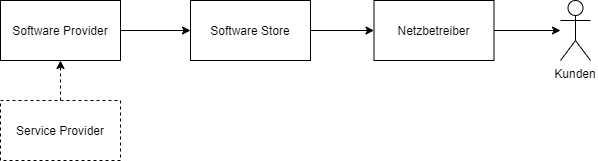
\includegraphics[width=0.8\columnwidth]{pictures/supplychain.png}
	\label{img:supplychain}
	\caption{Supply Chain von Software}
\end{figure}
Da ein Software Store viele Aufgaben mit sich bringt, wird im folgenden ein Konzept einer Wertschöpfungskette für diesen erstellt, welche eine detaillierte Sicht des Software Stores bieten wird. Nach der Wertschöpfungskette von Porter sind Unternehmen in primäre und unterstützende Aktivitäten aufzuteilen.\footnote{quelle} Primäre Aktivitäten "liefern dabei einen direkten wertschöpfenden Beitrag zur Erstellung eines Produktes."\footnote{https://refa.de/service/refa-lexikon/wertschoepfungskette, 21. Mai 2020} Unterstützende Aktivitäten sind als "notwendige Voraussetzung zu Erstellung der Produkte"\footnote{ebd.} zu sehen. Abbildung \hyperref[img:wsk]{8} gibt einen Überblick der identifizierten Bausteine der einzelnen Aktivitäten, welche im folgenden genauer dargestellt werden. Im Rahmen der Erstellung des Business Model Canvas wurde bereits ein Unterteilung in unterschiedliche Aufgabenbereiche vorgenommen \textit{(Kap. \ref{key_activities})}, welche im folgenden für die Gruppierung der Bausteine verwendet wird.
\subsubsection{Primäre Aktivitäten}
%Todo: Gruppierung der Bausteine nennen, wie i absatz zuvor beschrieben
\textbf{Eingangslogistik}\\
Im Kontext der Eingangslogistik muss die \textbf{Verifikation} eingehender Softwares und die anschließende \textbf{Aufnahme in den Shop }erfolgen. Die veriZur erfolgreichen Verifizierung müssen die \textbf{Sicherheitskriterien} des Shops müssen eingehalten werden. Ist dies der Fall, wird die Software den Aufnahmeprozess durchlaufen, welche im Rahmen der Operationen durchlaufen wird.\\\\
\textbf{Operationen}\\
Der Aufnahmeprozess einer Software in den Shop startet mit einer \textbf{Klassifizierung von Software}. Im Rahmen dieser werden Softwares anhand von Faktoren bewertet die Fahrzeughalter bei der Entscheidungsfindung zwischen Softwares unterstützen sollen. In Kapitel \ref{sw_klassifizierung} wird ein mögliches Konzept vorgestellt.\\
Neben der Klassifizierung von Software ist die Stetige (Weiter-)Entwicklung  des Shops notwendig. Diese sollte, wie im Forschungsseminar skizziert, im Kontext der Prinzipien des UCD erfolgen. Durch die stetige Wartung soll ein Absturz des Shops verhindert werden und Lücken in der Architektur identifiziert werden. 
\\\\
\textbf{Marketing \& Vertrieb von Produkten}\\
noch 1,5 Seiten, gogogo\\
SW vorschlagen: SUPR\textit{(SW finden)}\\
Angebotsunterbreitung: SUPR\textit{(moment des Angebotsunterbreitung)}\\\\
\textbf{Ausgangslogistk}\\
Gesicherter Download: Uptane\\\\
\textbf{Kundendienst}\\
Autmoatische Erkennung von Software Bedarf: OpenScenario\\

\begin{figure}[!h]
	\hspace{-1cm}
	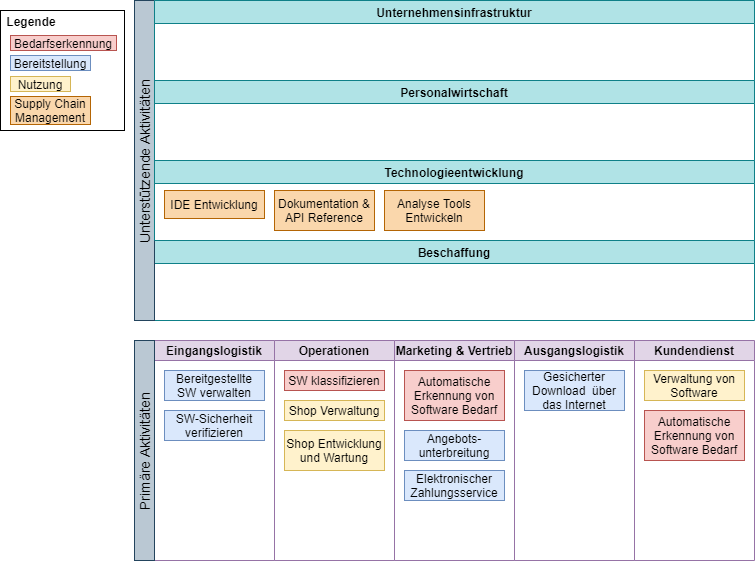
\includegraphics[width=\columnwidth]{pictures/wsk.png}
	\label{img:wsk}
	\caption{Die wichtigsten Bausteine einzelner Aktivitäten}
\end{figure}
\subsubsection{Unterstützende Aktivitäten}


WSK/SC vorstellen und Aktivitäten erklären.\\
EInzelne Aktivitäten durchgehen Bausteine einfügen\\
WSK Aktivitätenzwischen Erkennung und Bereitstellung aufteilen(?)

wichtige Bausteine der WSK (erkennung und Bereitstellkung von SW)\\


Beteiligte Stakeholder der WSK\\
OEM \\
Datenanalyse, Bedarfsentdeckung und ServerSchnittstelle\\
Softwareprovider\\
Softwareentwicklung, Bedarfsentdeckung \\
ServiceProvider\\
Vollstrecker der eigentlichen DIenste (bei Services)\\
Konzept einer (modernen) Wertschöpfungskette\textit{ (eher eine SupplyChain)}\\
Primäraktivitäten sind der Erkennung bzw. der Bereitstellung zuzuordnen\\\\
\textbf{Erkennung}: \\
	Einkauf \& Lagerung\\
	Produktion\\\\
\textbf{Bereitstellung}:\\
	Marketing\\
	Lieferung\\
	Service\\

\textbf{Unterstützende Aktivitäten (Entlang der Erkennung Bereitstellung):}\\
	Unternehmensinfrastruktur\\
	Personalwirtschaft\\
	technologieentwicklung\\
	Beschaffung\\